\documentclass[11pt,a4paper]{article}

\usepackage[T1]{fontenc}
\usepackage[utf8]{inputenc}
\usepackage{mathptmx}
\usepackage{courier}
\usepackage[protrusion=true,expansion=false]{microtype}
\usepackage[margin=21mm]{geometry}
\usepackage{xcolor}
\usepackage{graphicx}
\usepackage{amsmath,amssymb}
\usepackage{booktabs}
\usepackage{longtable}
\usepackage{array}
\usepackage{caption}
\usepackage[section]{placeins}
\usepackage[numbers,sort&compress]{natbib}
\usepackage[colorlinks=true,linkcolor=blue!50!black,citecolor=blue!50!black,urlcolor=blue!50!black]{hyperref}

\graphicspath{{figures/}}
\captionsetup{font=small,labelfont=bf}
\setlength{\parskip}{0.2em}

% Section references into reports/ml_nature.md. [S n] in the text means
% section n of that file; the summary (reports/ml_nature_summary.md)
% carries one paragraph per section with the regenerate command.
\renewcommand{\S}[1]{[\textsection\,#1]}
\newcommand{\code}[1]{\texttt{#1}}

\title{What machine learning taught us about the open stacks problem,\\ and what it did not}
\author{Alexandre Linhares\thanks{The analyses reported here were carried out
with Claude Code in unattended loops; see ``How this work was done'' in
Section~\ref{sec:intro}. Every number in the paper is copied from a numbered
section of the project's findings file and regenerates by a named command
(Appendix~\ref{app:provenance}).}}
\date{28 September 2026}

\begin{document}
\maketitle

\begin{abstract}
The minimization of open stacks problem (MOSP) asks in what order to make a
set of products so that the number of customer orders open at any one time is
as small as possible. It is NP-hard, and it is equal to a classical graph
quantity: the pathwidth of a graph on the customers, plus one. Over four
unattended analysis loops we pointed machine learning and large-scale
measurement at a corpus of 6,376 instances with certified optimal values and
at 51,000 generated instances. Learning never made the solver faster: three
learned components (bounds, branching, imitation) each resolved into a
statement about the solver or the problem instead. What the measurements
established is more useful. The optimum is sandwiched between two textbook
graph numbers, both now proved theorems; the best point estimate is a
treewidth heuristic; the solver's proved lower bound fails for a structural
reason that no formula over the usual invariants can repair. Hardness has a
sharp ridge at a simple density condition, grows exponentially along it, and
depends on the labelled graph and on nothing else in the matrix. The
imitation ranker distilled into a one-sentence closing rule that beats it.
A differential harness found a false refutation the verification machinery
could not see, and every refutation at 40 customers or fewer now carries a
certificate a third party checks in milliseconds. The paper states what size
range each claim covers, which of the pre-registered kill criteria were met,
and what remains unchecked at $125 \times 125$.
\end{abstract}

\section{The problem, and why it is a graph problem}
\label{sec:intro}

\paragraph{The problem.}
A factory has a list of products to make and a list of customers. Each
customer wants some subset of the products. A customer's \emph{stack} opens
when the first product they want is made and closes when the last one is
done. Products are made one at a time, in some order. The question is which
order keeps the largest number of simultaneously open stacks as small as
possible. That number, minimised over all orders, is the instance's
\emph{optimum}. The problem is NP-hard \citep{LY2002}. The input is a 0/1
matrix with one row per customer and one column per product.

\paragraph{The graph.}
Draw one vertex per customer and join two customers whenever they share a
product. Every product then becomes a \emph{clique} (a set of vertices all
joined to each other), and the graph is a union of cliques. This is the
\emph{MOSP graph} of \citet{Yanasse1997a}, and the optimum depends only on
it: two matrices with the same MOSP graph have the same optimum. The
literature also uses a second graph, with a vertex per product and an edge
between products that share a customer; \citet{YanasseSenne2010} call the two
``completely different'' and use the second one for one purpose only,
splitting an instance into independent parts.

\paragraph{Pathwidth.}
A \emph{path decomposition} of a graph is a sequence of overlapping vertex
sets (``bags'') laid out along a line, such that every edge has both ends in
some bag and the bags containing any one vertex form a contiguous stretch.
Its width is the size of the largest bag minus one, and the \emph{pathwidth}
of the graph is the least width of any path decomposition. An equivalent
picture is \emph{vertex separation}: order the vertices left to right, and at
each cut count the vertices on the left that still have a neighbour on the
right; the vertex separation number is the smallest achievable maximum count.
\citet{Kinnersley1992} proved the two are equal. \emph{Treewidth} is the same
construction with the bags arranged along a tree instead of a line; it is
never larger than pathwidth.

\paragraph{The chain.}
The equality between open stacks and pathwidth rests on four published steps.
MOSP is the same problem as gate matrix layout, a VLSI problem, by definition
\citep{LY2002}, whose interval-graph reading goes back to \citet{Ohtsuki1979},
\citet{Wing1985} and \citet{Mohring1990}; gate matrix layout cost equals
pathwidth plus one \citep{FL1989}, through a column-expansion lemma
\citep{FL1987} that is \citeauthor{Yanasse1997a}'s clique-per-product graph in
matrix vocabulary; pathwidth equals vertex separation \citep{Kinnersley1992},
whose NP-completeness is due to \citet{Lengauer1981}; and the graph in
question is the MOSP graph \citep{Yanasse1997a}. Related search-game
formulations are in \citet{KirousisPapadimitriou1986}. So:
\[
\text{optimum} \;=\; \text{pathwidth(MOSP graph)} + 1
\;=\; \text{vertex separation(MOSP graph)} + 1 .
\]

\paragraph{We had the two graphs swapped.}
For part of its life the project attached this theorem to the product graph.
Measured against published optima it undercounted, which was read as a gap in
the reduction; it was a consequence of testing the wrong graph. The mistake
went further than the code. The Lean~4 development's original statement of
the reduction was over the product graph too, and over that graph the
statement is false: one product shared by four customers, each with a private
product of their own, has optimum 4, while its product graph is a star with
pathwidth 1. That counterexample is now a Lean theorem, the false statements
are deleted, and the equality above is a \code{sorry}-free theorem in both
directions over the MOSP graph \S{26}. Two more statements in the development
turned out to be false rather than hard: a ``branch lemma'' that asked for
neither connectivity nor attachment, refuted by four isolated vertices
\S{39}. The corrected lemma and its separator form are proved \S{39, 40}. At
the end of the work the development holds 34 named theorems and one
\code{sorry}, kept on purpose as a stated conjecture \S{40}. The lesson we
record is that a stated-but-unproved theorem needs a small-instance check
before it is committed.

\paragraph{How this work was done.}
The analyses were carried out with Claude Code in four unattended loops, one
item per fresh session, each item an immutable question with a pre-registered
kill criterion, a progress file and a report section as its deliverable. The
first plan asked ten questions (findings \S{1--14}), the second eleven
(\S{15--27}), the third seven (\S{28--40}). Every number in this paper is
copied from the section it cites and regenerates by a command named there;
Appendix~\ref{app:provenance} lists them. The paper computes nothing new.
Section references of the form \S{$n$} point to the findings file; citations
in the usual form point to the literature.

\section{The corpus and the instruments}
\label{sec:corpus}

\paragraph{What ``certified'' means.}
A \emph{witness} is a production order that achieves a value $k$; it is
checked by simulating the order and counting stacks, which anyone can do. A
\emph{refutation} is a proof that no order achieves $k-1$. An optimum is
\emph{certified} when it has both, or when a proved lower bound already
equals $k$. The corpus holds 6,376 instances at 9 to 134 customers, every one
with a certified optimum and a witness, drawn from the standard benchmark
collections (Harvey, Simonis, Faggioli--Bentivoglio, Chu \& Stuckey, Shaw,
Wilson, SCOOP, Challenge) \S{1}.\footnote{Two $125 \times 125$ entries had
their optimality claims withdrawn after the bug of Section~\ref{sec:solver}
and are being re-certified; their values remain verified upper bounds
\S{35}.} The lopsidedness matters: 5,938 of the 6,376 have 30 or fewer
customers, and the class that costs a day of compute is 25 rows \S{28}.

\paragraph{The corpus is smaller than it looks.}
Two instances with the same MOSP graph up to renaming have the same optimum.
Counted by graph, the 6,376 instances hold 3,667 distinct graphs; 42.5\% of
the corpus is isomorphic copies, and 1,669 instances (26.2\%) are complete
graphs whose optimum is trivially the number of customers \S{1}. 157 graph
classes span more than one benchmark file, so a train/test split by file
leaks copies across the split; every split in this work groups by file and
by isomorphism class together \S{1}. That leak was later measured: it was
worth about a seventh of a learned heuristic's recorded gain \S{28}.

\paragraph{The generators are fingerprintable.}
A random forest on 28 structure-only features assigns 94.4\% of instances to
the collection that generated them with the source file held out, and
98.8\% among instances of equal size where chance is 61.6\% \S{2}. The
fingerprint can be stated in two lines: every Harvey instance has constant row
or column sums and no other generator's does; Faggioli--Bentivoglio caps the
largest product at half the customers; Chu \& Stuckey is sparse where nothing
else is \S{2}. Figure~\ref{fig:space} shows the instance space: a lattice of
74 size cells with empty regions between, and the 24 industrial SCOOP
instances in the same sparse corner as all 200 Chu \& Stuckey instances
\S{2}. A result on one collection is a result about that generator.

\begin{figure}[t]
\centering
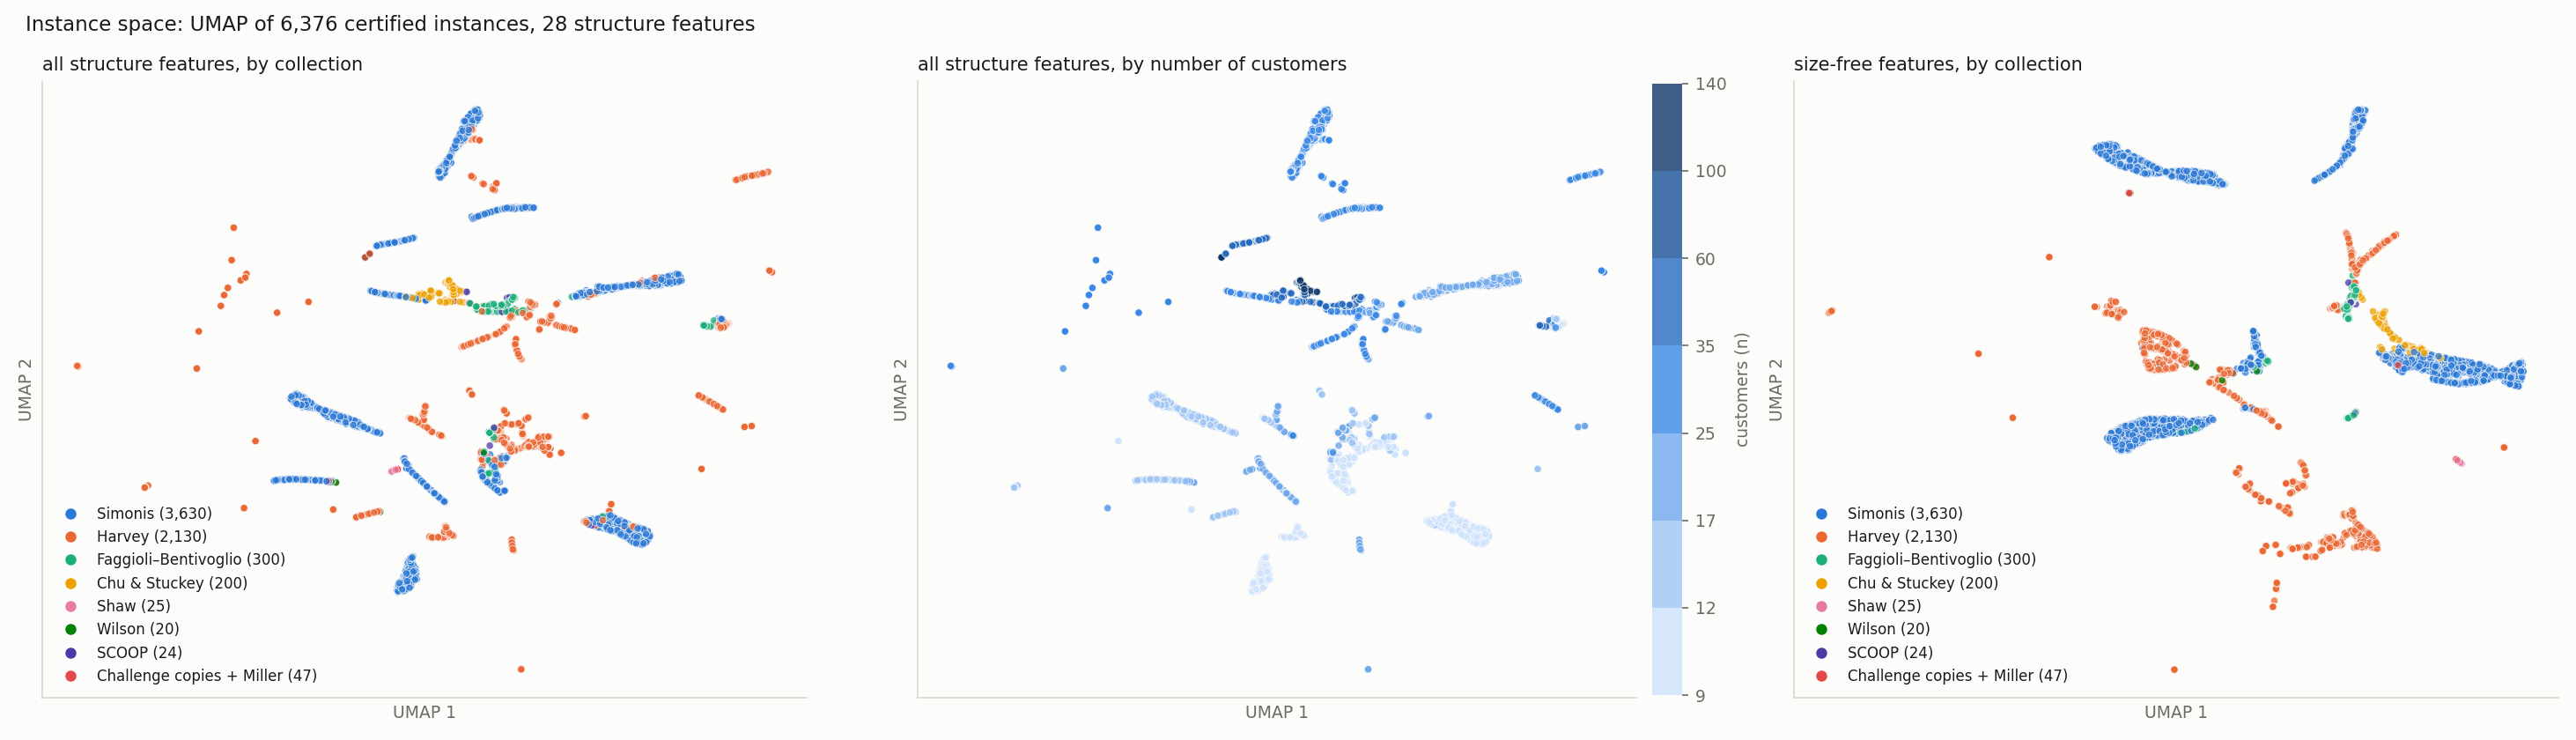
\includegraphics[width=\textwidth]{instance_space}
\caption{The instance space of the corpus, a UMAP embedding of 6,376
instances on 28 structure features, coloured by collection (left), by number
of customers (middle) and by collection again on size-free features (right).
The map is a lattice of streaks, one per $(n,m)$ size cell, not a continuum;
within a streak the generators separate. Chu \& Stuckey and the industrial
SCOOP instances share the sparse corner \S{2}.}
\label{fig:space}
\end{figure}

\paragraph{The generated campaign.}
Small instances are free: at 40 customers a random instance is generated,
solved and refuted in a fraction of a second. So the questions about density
were asked on ensembles we control. The campaign holds 37,800 instances in
252 cells (10 to 40 customers, products equal to or twice the customers, two
generators, 150 per cell), every one certified and refuted under both search
configurations, for 2.16 core-hours \S{9, 10}. It was then extended upward:
6,747 certified instances at 50--75 customers \S{16}, 2,750 at other product
ratios \S{25}, 3,378 more at 40--100 \S{37}, and one 25-instance cell at 100
customers on the hardness ridge, of which one instance certified \S{34}.
Every instance regenerates byte for byte from its seed.

\paragraph{Nodes, not seconds.}
The complete search of \citet{ChuStuckey2009}, which the solver runs, visits
search \emph{nodes}: partial closing orders. Node counts are the unit of
hardness throughout. At 40 customers or fewer the refutation is 0.5--0.7\% of
the wall-clock cost, seconds are a smooth function of size alone, and node
counts vary by three orders of magnitude across cells at fixed size, so at
these sizes the clock does not see hardness at all \S{10}. On a loaded
machine the clock also invents speed-ups: in one study seconds spread
$1.49\times$ where nodes spread $1.05\times$ \S{18}. Every node count is
dated against the version of the search that produced it, because a pruning
rule changed mid-way (Section~\ref{sec:solver}).

\paragraph{The rules.}
Four rules held for all four loops. A prediction is never a bound: nothing
learned reaches the code that decides which $k$ to try, because a lower bound
one too high makes the solver return a wrong answer whose witness still
verifies. Every split groups by file and isomorphism class. Every claim states
its size range, and nothing below 100 customers is evidence about
$125 \times 125$ except through an extrapolation that says so. No solver
default was changed by a loop; the one code change that altered an answer,
the bug fix of Section~\ref{sec:solver}, went through the owner.

\section{What determines the optimum}
\label{sec:optimum}

\paragraph{The best point estimate is a treewidth heuristic.}
Thirteen pathwidth-adjacent graph invariants were added to the feature
table. One carries almost everything: the min-fill treewidth heuristic plus
one. Table~\ref{tab:estimate} compares it with the solver's own proved
bounds. It is exact on 85.7\% of the corpus, better than either bound, and
leads in every size band up to about 50 customers; at 125 it is off by 4.2
stacks on average and inside its $\pm 1$ band on 2 of 25 instances \S{4, 14}.
It is a bound on nothing: it sits below the optimum on 481 instances and
above on 428 \S{4}. On the residual over the proved bound the whole group of
invariants adds nothing (grouped MAE $-0.004$): they know what the bound
knows, expressed differently \S{4}.

\begin{table}[t]
\centering
\small
\caption{Point estimates of the optimum over the whole corpus (9--134
customers, 6,376 instances). MAE is mean absolute error in stacks. The
treewidth heuristic is not a bound \S{4}.}
\label{tab:estimate}
\begin{tabular}{lrr}
\toprule
estimate & exact & MAE \\
\midrule
min-fill treewidth $+1$ & 85.7\% & 0.188 \\
solver's upper bound (heuristic) & 84.6\% & 0.239 \\
solver's lower bound (proved) & 77.0\% & 0.431 \\
\bottomrule
\end{tabular}
\end{table}

\paragraph{A sandwich, now two theorems.}
Two textbook graph numbers bracket the optimum on every instance we have.
The \emph{degeneracy} of a graph is the largest $d$ such that some subgraph
has every vertex of degree at least $d$. A \emph{bandwidth} estimate
(reverse Cuthill--McKee) is the longest edge when the vertices are laid on a
line by that heuristic. On all 6,376 instances,
\[
\text{degeneracy} + 1 \;\le\; \text{optimum} \;\le\; \text{bandwidth}_{\mathrm{rcm}} + 1,
\]
with the two ends coinciding, and so forcing the optimum, on 2,823 instances
\S{5, 26}. Both inequalities are proved in the Lean development for every
finite graph, through vertex separation and Kinnersley's equality, and since
the equality of Section~\ref{sec:intro} is itself proved they are theorems
about the optimum rather than about pathwidth \S{26}. Treewidth plus one is
a lower bound by the same route, proved through a lemma that Mathlib lacked,
that the path graph is a tree \S{39}. Where the two ends differ, the
optimum's position between them is not a constant: pooled over the corpus it
sits at the midpoint, but by density it runs from the bottom below 1.5
customers per product to two thirds of the way up above 6 \S{5, 12}.

\paragraph{Where the proved bound fails, and why.}
The solver's lower bound is the best of four components: a trivial bound, a
clique bound, contraction degeneracy \citep{BKW2006}, which is the
arc-contraction bound of \citet{YBS1999} under another name, and a
neighbourhood-expansion bound. It equals the optimum on 77.0\% of the
corpus, misses by one on 17.7\%, and by two or more on 338 instances (5.3\%;
51.0\% of Chu \& Stuckey) \S{6}. A gap of two never occurs below 20
customers \S{6}. The reason is structural, not statistical. Three of the
bound's components are really bounds on \emph{treewidth}, and on about half
of the 338 gap instances pathwidth is provably larger than treewidth
(Table~\ref{tab:gap}), so no tuning of those components could ever close the
gap \S{6, 21}. The instances look like small cliques glued at a few hub
customers into a branching tree, with a fringe of customers who want a single
product \S{6}.

\begin{table}[t]
\centering
\small
\caption{The 338 corpus instances where the proved lower bound is two or more
below the optimum, by whether pathwidth exceeds treewidth. Exact treewidth was
computed to 26 vertices by subset dynamic programming and to 64 by a budgeted
decision search; ``open'' means the search returned an interval \S{21}.}
\label{tab:gap}
\begin{tabular}{lrr}
\toprule
 & instances & share \\
\midrule
pathwidth $>$ treewidth (bound structurally blocked) & 164 & 48.5\% \\
pathwidth $=$ treewidth & 80 & 23.7\% \\
open (82 of them above 64 customers) & 94 & 27.8\% \\
\bottomrule
\end{tabular}
\end{table}

\paragraph{The smallest such graph has ten vertices.}
A bit-flip search with the exact solver as oracle found a 10-vertex, 21-edge
graph, three $K_4$s glued pairwise at three hub vertices plus a tenth vertex
joined to one non-hub of each, with treewidth 3 and pathwidth 5, and proved it
vertex- and edge-minimal for a gap of two \S{21}. A census then settled the
question by exhaustion: over all 287,884 graphs on at most 9 vertices the
gap is 0 or 1; exactly four graphs on 10 vertices have gap 2, all one family;
1,034 on 11 have it and none has gap 3, so gap 3 needs at least 12 vertices
\S{27}. Twelve of the 1,034 have treewidth 2 and pathwidth 4 with no $K_4$
at all, three triangles strung between two poles: a second shape, not a tree
of cliques, that any pathwidth bound must see \S{27}.

\paragraph{No formula and no branching rule fixes it.}
Exact treewidth plus one beats the solver's certified bound on 933 corpus
instances (14.6\%) and on 199 of the 338 gap instances \S{24}. Beyond that,
nothing was found. A search over 11,589 two-invariant formulas on 30
branching-aware invariants left 47 survivors, 36 of which were treewidth plus
one restated; 77\% of fitted candidates leaked on a grouped hold-out, because
a constant fitted on 51,000 instances is the maximum of a sample; no
candidate beat $\max(\text{bound}, \text{treewidth}+1)$ on more than 0.1\% of
the instances with exact treewidth \S{24}. A harness that takes any candidate
bound as a function, checks it on 49,862 certified instances, attacks it with
11,880 adversarial evaluations and scores it on the gap instances was then
built \S{38}. Three branching-aware candidates, resting on the branch lemma
of \citet{FL1987} and \citet{Kinnersley1992} and its separator
generalisation, went through it: all valid, all survived the adversary, and
by branching none beat the reference on any gap instance; the kill criterion
(none beats the reference on more than 5\% of gap instances) was met at
0.0\,/\,0.0\,/\,2.4\% \S{38}. The next bound idea has to be a different
pathwidth argument.

\paragraph{On random instances the optimum concentrates.}
At every one of the 36 cells at 40 customers the coefficient of variation of
the optimum is under 0.2 (median 0.031); a cell is two or three adjacent
integers \S{12}. The mean is a straight line in the number of customers at
fixed degree, with $r^2 \ge 0.999$ in all 17 fixed-degree series \S{12}
(Figure~\ref{fig:concentration}). A closed-form fit for that mean has
held-out error 0.49 stacks on the 252 cell means, and it is an estimate of a
mean, never a bound: per instance it sits below the optimum on 9,445 and
above on 10,641 \S{12}. Its constants break with size. On Chu \& Stuckey's
instances from 30 to 125 the line holds but the intercept and slope do not,
so the bias grows to $+8.1$ stacks on the sparsest 125-customer class while
staying within $\pm 2$ at densities 4--10 \S{14}. Every confidence interval
calibrated at 40 customers or fewer fails by 50--75 and is not to be quoted
at 50 or more; that kill criterion was met for every interval \S{14}.

\begin{figure}[t]
\centering
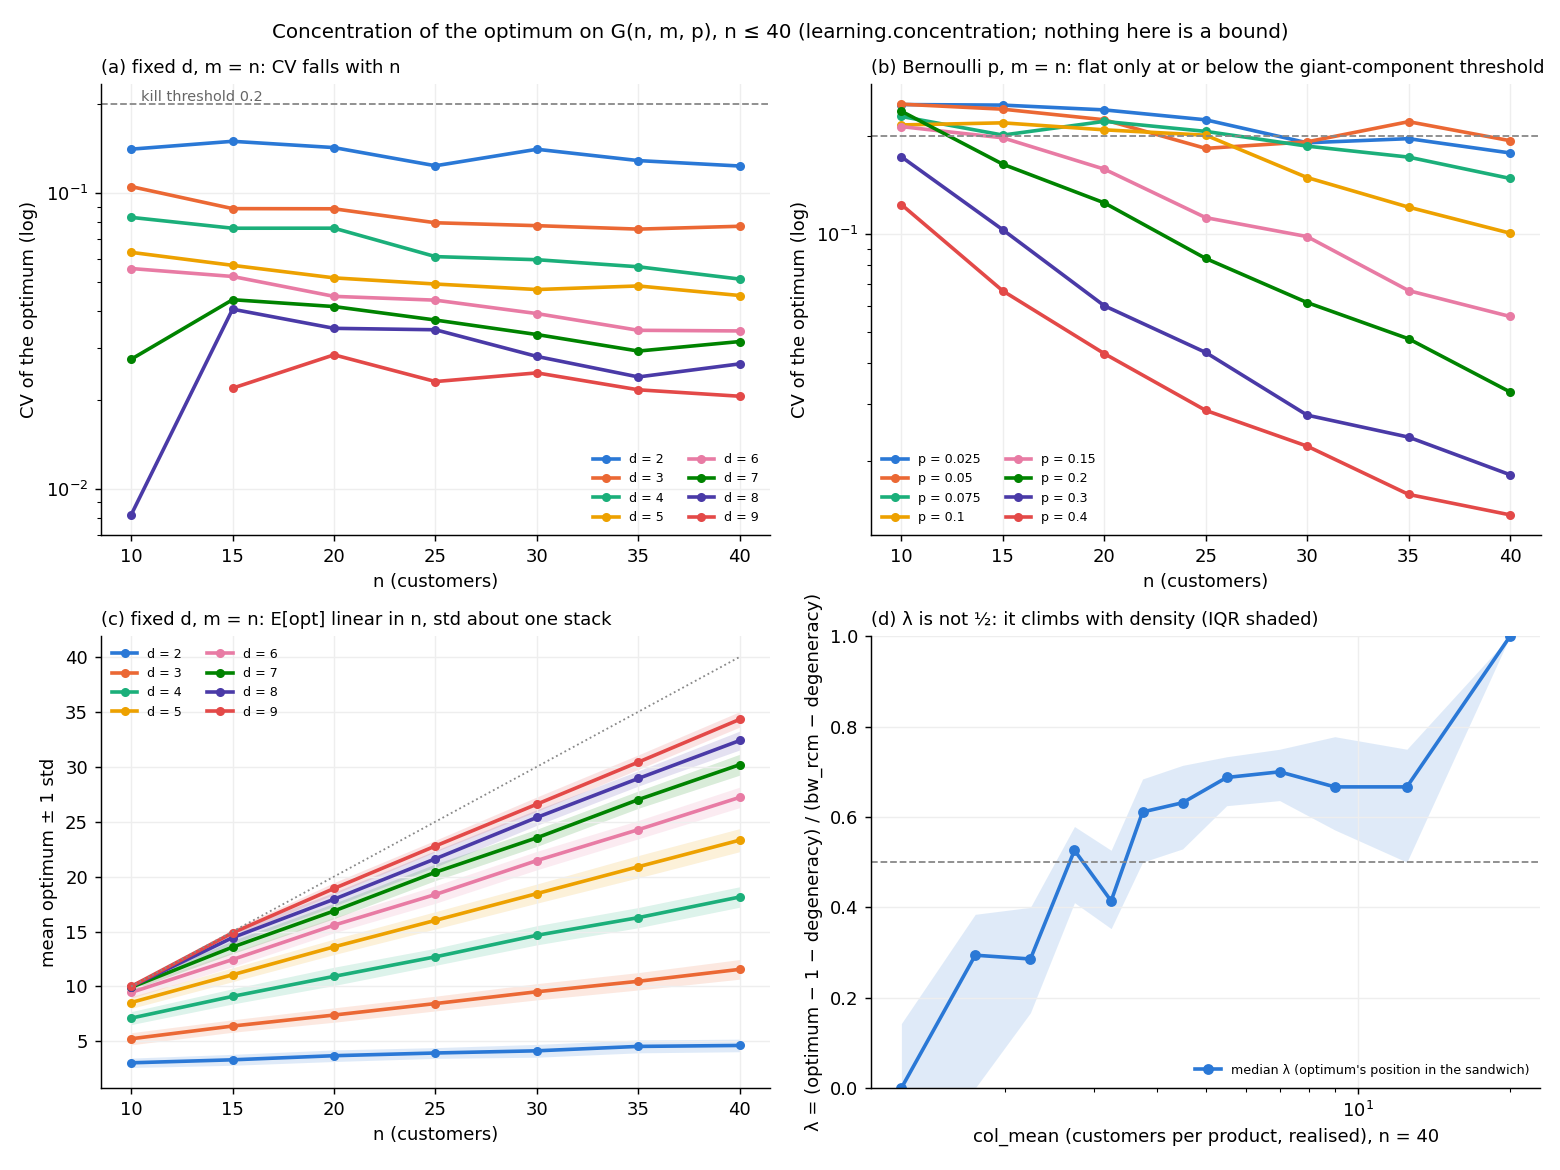
\includegraphics[width=0.74\textwidth]{concentration}
\caption{Concentration of the optimum on generated random instances at 10--40
customers. (a) At fixed customers per product the coefficient of variation
falls with size; (b) under Bernoulli sampling it stays flat only at or below
the giant-component threshold; (c) the mean optimum is a line in $n$ with a
standard deviation of about one stack; (d) the optimum's position in the
sandwich climbs with density and is not one half. Nothing here is a bound
\S{12}.}
\label{fig:concentration}
\end{figure}

\section{What makes an instance hard}
\label{sec:hardness}

\paragraph{There is a ridge.}
Figure~\ref{fig:ridge} is the one picture the rest of this section explains.
At every size from 15 to 40, in both generators, the median number of nodes
to refute $\text{optimum}-1$ rises and falls with density by two orders of
magnitude each side of a peak at 40 customers, and the peak sharpens with
size \S{11}. On the ridge the median grows exponentially at 0.086--0.105
$\log_{10}$ nodes per customer, doubling every 2.9--3.5 customers, with a
power law ruled out at 5--10 times the residual; off the ridge growth is
exponential too but slower, doubling every 4.5--4.9 customers \S{11}. The
ridge sits at about three customers per product when products equal
customers and two when products are twice the customers \S{11}. Chu \&
Stuckey's ``density 2'' classes, the ones that take a day at
$125 \times 125$, are the peak cell at both 30 and 40 customers, and their
density 4 is its dense shoulder \S{11}.

\begin{figure}[!tb]
\centering
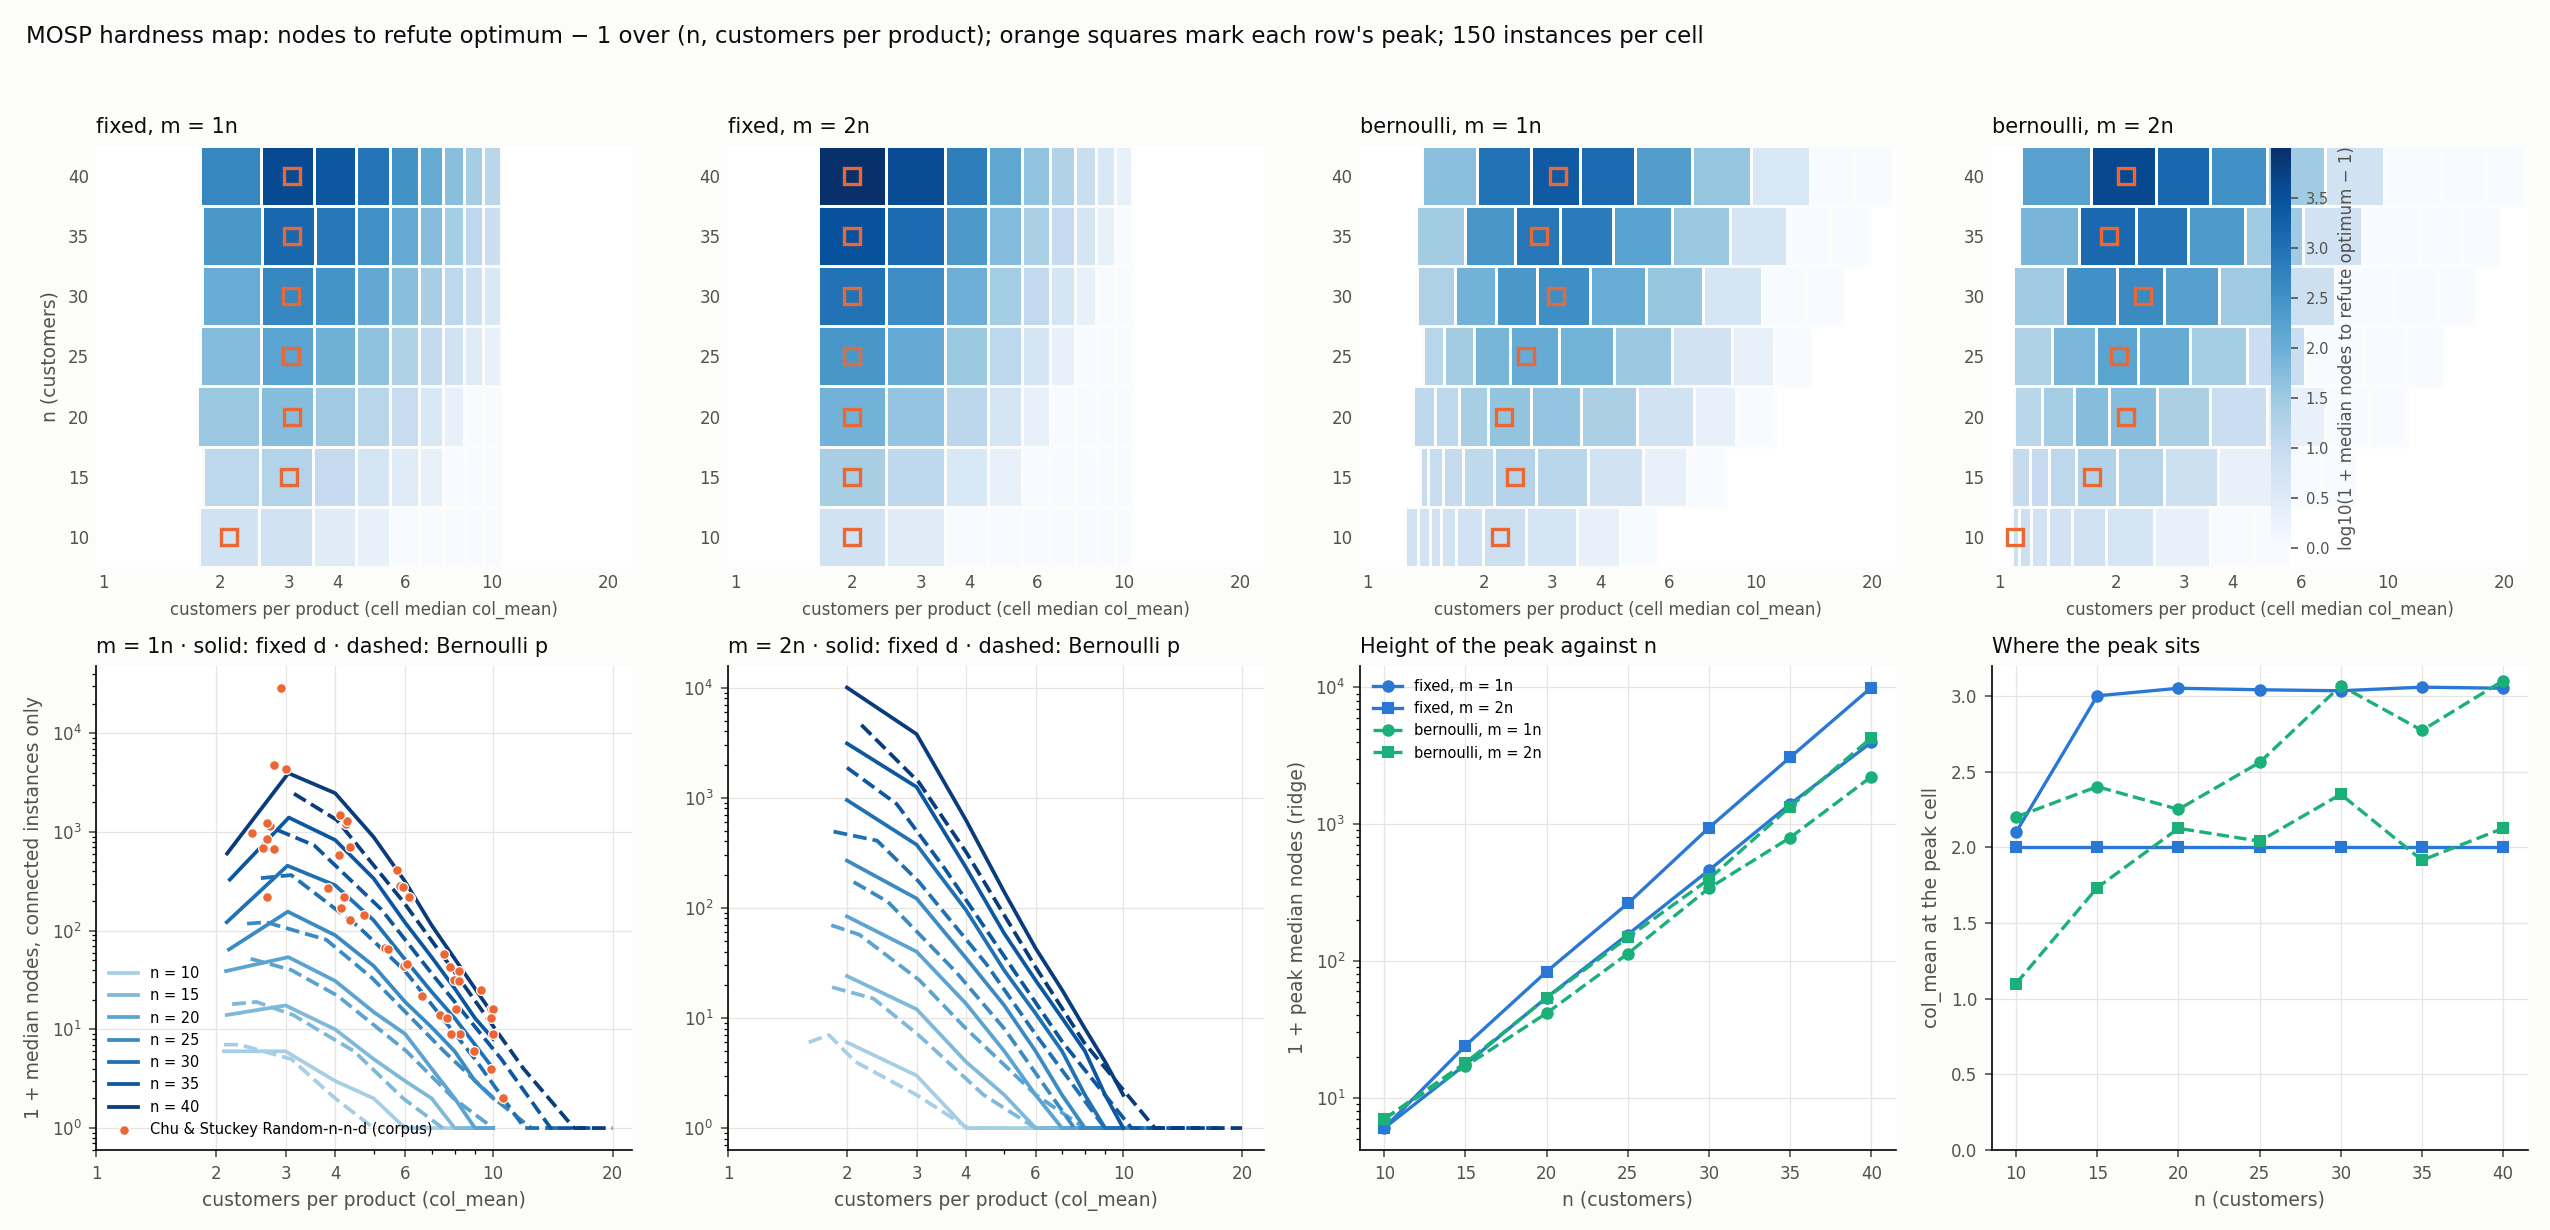
\includegraphics[width=\textwidth]{hardness_map}
\caption{The hardness map. Top: median $\log_{10}$ nodes to refute
$\text{optimum}-1$ over (customers, customers per product) for two
generators and two product ratios, 150 instances per cell, with each row's
peak marked. Bottom left: the same at $m=n$ as curves, with Chu \& Stuckey's
corpus instances at 30 and 40 customers overlaid; they sit on the peak.
Bottom right: the peak's height grows exponentially in $n$ and its location
is fixed \S{11}.}
\label{fig:ridge}
\end{figure}

\paragraph{The growth rate fell, and then did not.}
Fitted at 40 customers or fewer, the ridge law pre-registered $5 \times
10^{11}$ nodes for a $125 \times 125$ ridge refutation; the two counts then on
record were $1.6$--$1.7 \times 10^{11}$, within a factor of three after eight
decades of extrapolation \S{11, 14}. The campaign to 75 customers found the
rate drifting down in 18 of 18 fixed-density series, by about 0.002 per
customer per ten customers, and a drift-corrected law put the figure at
$1.5 \times 10^{11}$ \S{16}. The 100-customer ridge cell contradicted the
drift: its refutations sit 0.5--0.7 decades above the drifting law's median,
and 24 of 25 did not finish in 2,400\,s each after $3.4$--$4.8 \times 10^9$
nodes \S{34}. Fitted as a censored cell, the rate over 75 to 100 is 0.116
[0.110, 0.121] per customer against 0.092--0.095 over 60 to 75 \S{35}. Read
like with like (the drift-corrected headline had compared a law for one
search configuration against counts from another), a constant-rate law
refitted on 10 to 100 gives Table~\ref{tab:rate}'s figure: a median of
$2.7 \times 10^{11}$ nodes and 55 hours on one core per $125 \times 125$
ridge refutation, with the record's three counts falling 0.2 decades either
side \S{35}. Every 125 figure is an extrapolation of 25 customers from a cell
that is mostly lower bounds. Figure~\ref{fig:scale} shows the fits against
the corpus counts.

\begin{table}[t]
\centering
\small
\caption{Successive predictions of the median node count for a
$125 \times 125$ ridge refutation (Chu \& Stuckey density 2), each from the
sizes it was fitted on. The last row is the one to quote; it is for the
search configuration before the bug fix of Section~\ref{sec:solver}, and
post-fix counts are at least $2.34\times$ larger on the 100 cell \S{35}.}
\label{tab:rate}
\begin{tabular}{llll}
\toprule
fitted on & law & prediction at 125 & section \\
\midrule
10--40 & constant rate & $5 \times 10^{11}$ & \S{11} \\
10--75 & drifting rate & $1.5 \times 10^{11}$ & \S{16} \\
10--100 & constant rate, like with like & $2.7 \times 10^{11}$ [2.3, 3.2]; 55\,h & \S{35} \\
\midrule
record & three counts, $\log_{10}$ nodes & 11.21, 11.22, 11.66 (law's median 11.43 [11.36, 11.51]) & \S{35} \\
\bottomrule
\end{tabular}
\end{table}

\begin{figure}[!tb]
\centering
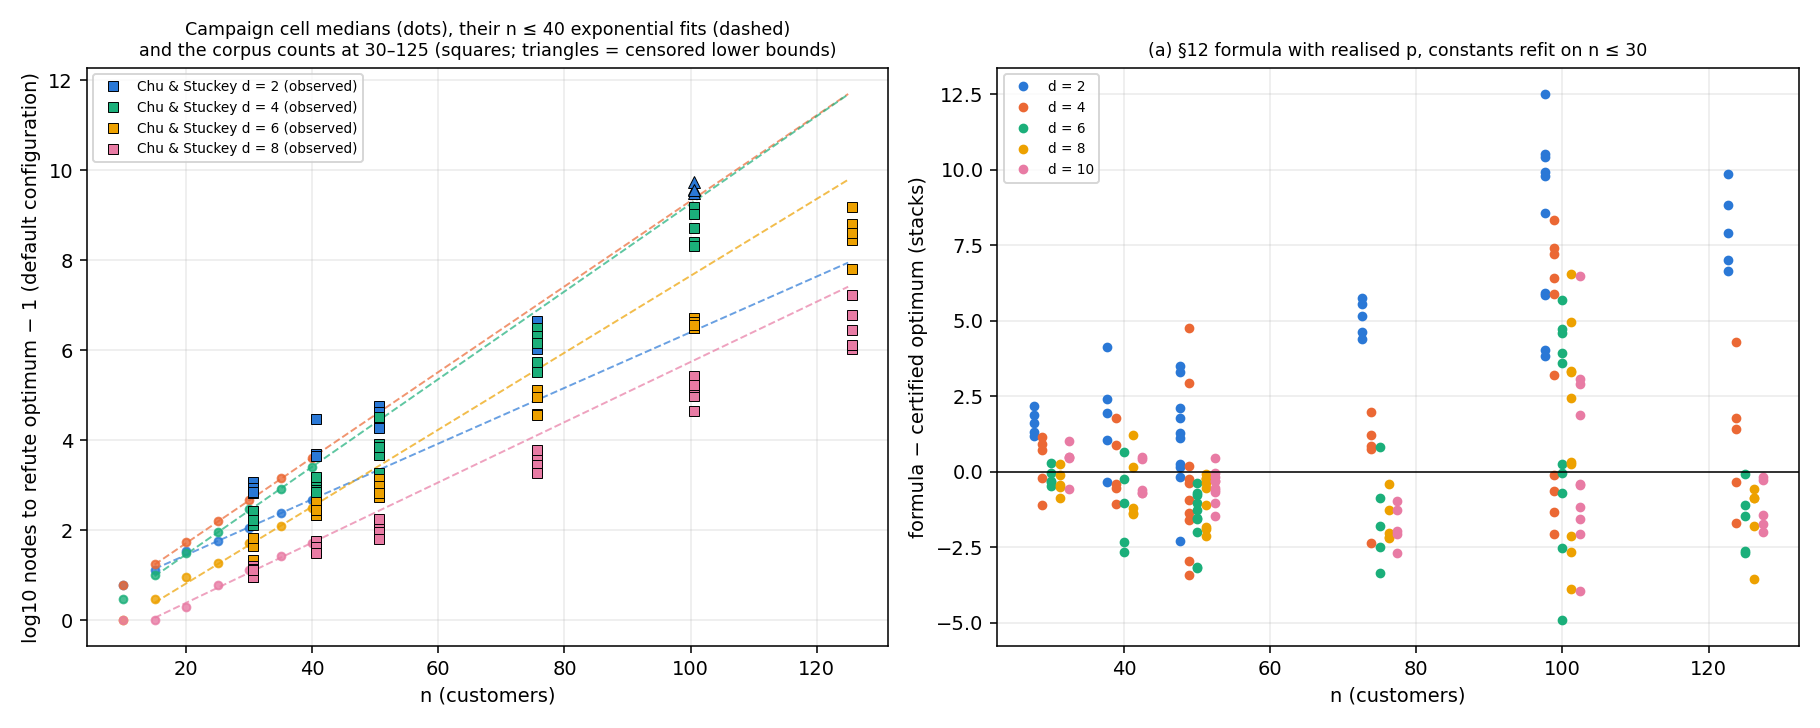
\includegraphics[width=\textwidth]{scale_test}
\caption{Do the small-size laws survive to 125? Left: campaign cell medians
at 10--40 customers with their exponential fits (dashed) against the corpus
counts at 30--125 (squares; triangles are censored lower bounds), by Chu \&
Stuckey density class. The forms hold; the fitted rates overstate the dense
classes and land within a factor of three on the two day-long ones. Right:
the mean-optimum formula's error grows linearly with size on the sparsest
class and stays within about $\pm 2$ elsewhere \S{14}.}
\label{fig:scale}
\end{figure}

\paragraph{Where the ridge is.}
The obvious coordinate, mean degree of the MOSP graph, is not it: the mean
degree at the peak runs from 3.9 to 37.6 as the product ratio goes from twice
the customers to an eighth of them \S{25}. The coordinate that is the same
across every ratio is the \emph{cover excess}, the number of ones in the
matrix minus the number of products, per customer: 2.0--2.5 at every fixed-
degree peak and 1.8--3.0 at every Bernoulli peak, the only candidate within a
factor of 1.65 across ratios \S{25} (Figure~\ref{fig:excess}). At excess 1
the customer--product incidence graph has as many edges as vertices; the
ridge is one independent cycle per customer. In customers-per-product terms
the ridge is at about $1 + 2.4\,n/m$ \S{25}. It is a density condition, not
a percolation threshold: the giant component of the incidence graph appears
0.34--0.78 decades below it, and no core or connectivity threshold coincides
with it at every ratio \S{36}. What it is a transition of is the search's own
state space: the number of closed customer sets \emph{reachable} from the
empty set through steps that fit the budget equals the node count to
0.03--0.06 decades at the median and peaks where the nodes peak \S{36}.

\begin{figure}[!tb]
\centering
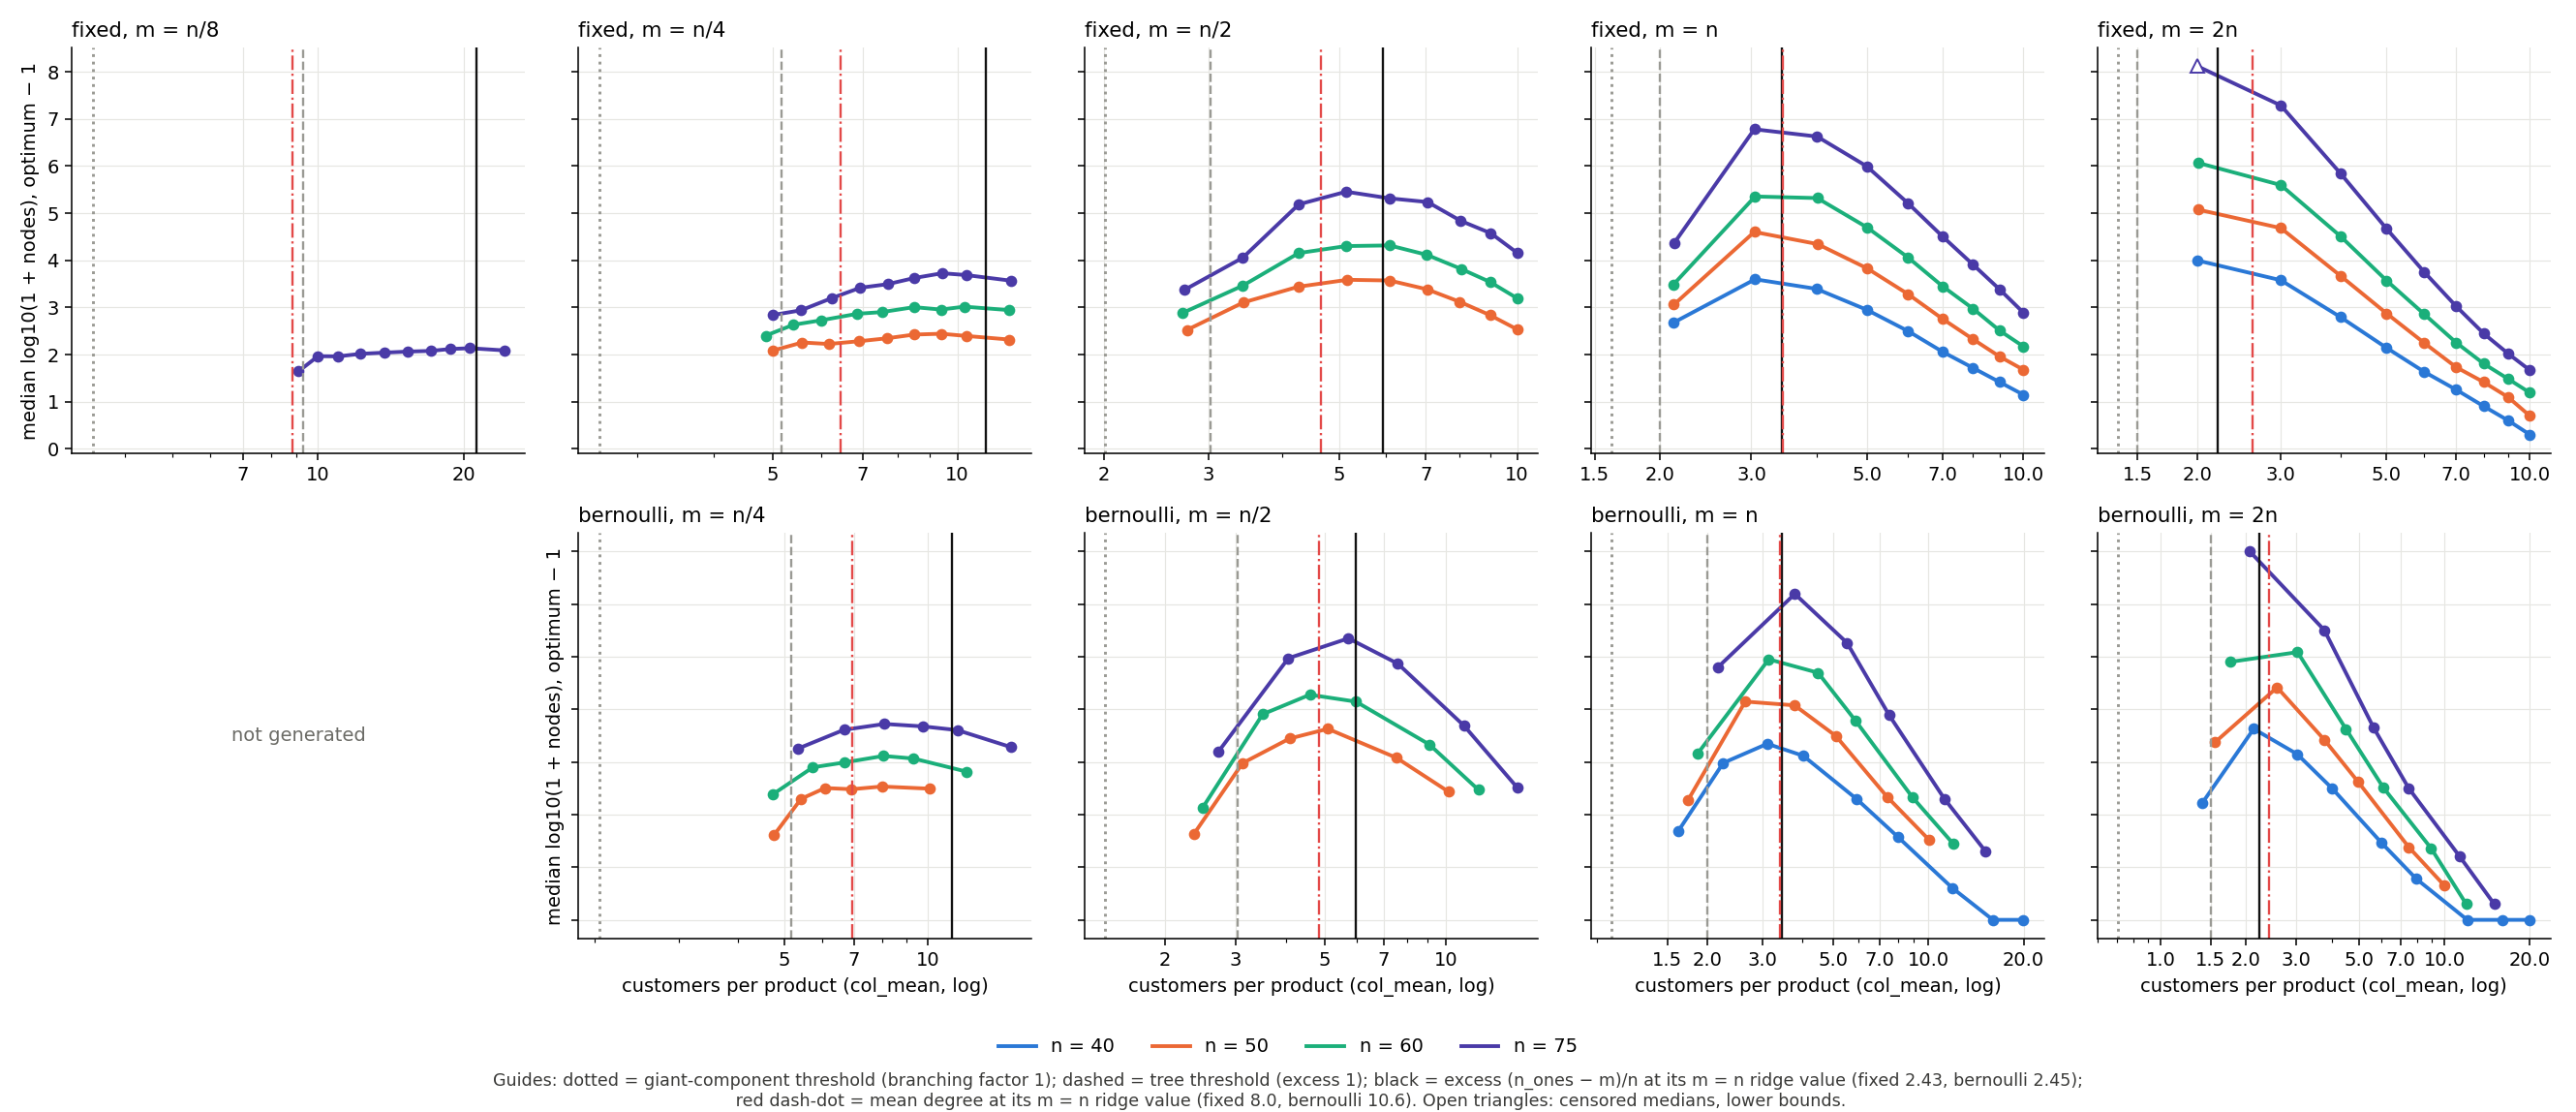
\includegraphics[width=\textwidth]{ridge_theory}
\caption{Why the ridge is where it is. Median $\log_{10}$ nodes against
customers per product at 40--75 customers, one panel per product ratio from
$m=n/8$ to $m=2n$. Vertical guides: the giant-component threshold (dotted),
excess 1 (dashed), mean degree calibrated at $m=n$ (red), and cover excess
calibrated at $m=n$ (black). Only the excess line lands on the peak in every
panel \S{25}.}
\label{fig:excess}
\end{figure}

\paragraph{How high the ridge is.}
The excess locates the ridge but says nothing about its height, which needs
the number of products separately. With 57 series peaks under each
configuration the law that survives is
$\log_{10}\text{nodes} \approx -0.10 + n\,(0.089 + 0.058 \log_{10}(m_{\mathrm{eff}}/n))$,
where $m_{\mathrm{eff}}$ counts products that carry an edge after dominance;
its in-sample error is 0.18 decades and 0.21 leaving a series out, and the
excess at the peak adds nothing to it \S{37}.

\paragraph{Only the labelled graph matters, for the search.}
Re-covering the same edge set with different products, 15,900 re-coverings of
1,400 instances, leaves the default node count \emph{exactly} unchanged in
every pair: the search reads neighbour masks and nothing else \S{13}. Graph-
only features predict nodes as well as graph plus matrix. What does move the
count is renaming the customers: 2--6\% at the median, up to $2.26\times$
under one configuration and $8.1\times$ under the other, the search's
tie-breaks and the floor for any label-free predictor \S{13}. For the SAT
path the story is different: re-covering moves the solver's conflict count by
$0.26$--$1.67\times$ between the 10th and 90th percentiles, in the direction
of the formula's clause count, with which conflicts correlate at Spearman
0.93--0.98 across instances \S{30}. Hardness is a property of the labelled
graph for the search and of the formula size for SAT.

\paragraph{The cost can be predicted within a decade.}
A censored regression in log space on label-free graph features, trained at
10--75 customers, puts 87.8\% of the 98 default-configuration counts and
89.3\% of the 103 other-configuration counts at 100--125 within one decade of
the truth, against 57.5--65.4\% and 59.2--61.2\% for the two earlier laws,
with a bias of $+0.4$ decades \S{19}. It sized the 100-customer ridge cell
correctly from the heuristic upper bound and under-predicted by 1.1 decades
from the certified optimum, because the optimum's fraction of $n$ is its
strongest term \S{34}. It is a prediction for ordering a queue, never a bound.

\section{What the solver learned about itself}
\label{sec:solver}

\paragraph{The two-key rule.}
The project had trained a LightGBM ranker to imitate the closing orders of the
witnesses, and it helped. Distilling it produced a rule a person can state:
\emph{close the customer that opens the fewest new stacks; on ties, the one
with the most unclosed neighbours} \S{7}. Table~\ref{tab:rule} compares it
with what it distilled from. The first key is the search's own cheapest-first
fan order, so the greedy is the search's first leaf; the tie-break is the
reverse of the textbook rule's \S{7}. Run over the whole corpus as the seed of
the restricted depth-first search, the rule beats the learned seed on every
statistic, and does so with no model, no training and no dependency, which
closed the question of whether LightGBM belonged in the solver \S{28}. It is
not the literature's heuristic under another name: the Minimal Cost Node
heuristic of \citet{BYS2004}, reimplemented from its pseudocode and
reproducing its worked example and 21 of 21 published values in
\citet{Frinhani2018}, shares the rule's first key on 98.8\% of its decisions
and has the opposite tie-break; the two produce the same closing order on
0.6\% of instances and the rule wins 592 to 242 where they differ \S{29}.

\begin{table}[t]
\centering
\small
\caption{Closing-order constructions, held out (1,920 instances, 9--134
customers, top) and as the seed of the restricted DFS over the whole corpus
(6,376, bottom). MAE and overshoot are in stacks above the optimum
\S{7, 28}.}
\label{tab:rule}
\begin{tabular}{lrrr}
\toprule
construction & MAE & exact & worst \\
\midrule
two-key rule & 0.348 & 80.7\% & $+9$ \\
LightGBM ranker & 0.519 & 75.0\% & $+34$ \\
MCN (textbook, node-closing) & 1.616 & 50.2\% & $+26$ \\
\midrule
DFS seed & mean overshoot & exact & ms per instance \\
\midrule
rule $+$ cs-dfs & 0.092 & 94.2\% & 16.7 \\
learned $+$ cs-dfs & 0.128 & 92.1\% & 20.6 \\
cs-dfs alone & 0.241 & 84.5\% & 29.5 \\
\bottomrule
\end{tabular}
\end{table}

\paragraph{Imitation is closed.}
Why did imitation learn so little? Because the target was mostly noise. Exact
path counting over the subset lattice shows the optimum is never unique: 0 of
2,812 corpus instances at 15 customers or fewer have a unique optimal closing
order, the median count is $4 \times 10^5$ at 10 customers and
$2.5 \times 10^{10}$ at 15, and about 90\% of the 2.27 million decisions the
ranker trained on were arbitrary choices among optimal ones \S{8}. With the
honest target, the \emph{set} of optimal moves at every state, and the rule's
own keys as features so that a model can only add to it, the best learned
policy beat the rule by 0.008 stacks against a kill threshold of 0.02; the
rule's pick was already in the optimal set at 99.71\% of states \S{23}.

\paragraph{Search rules measured, none enabled.}
Three proposed changes to the search were each measured behind a flag and
left off. Trying equal-cost candidates by degree instead of by index changes a
refutation's node count by 0.0\% at every size, because the pruning rules are
properties of the state and not of the order the candidates are read in; it
helps only the cheap satisfiable side, by 35\% of witness nodes at 75
customers \S{20}. A portfolio of sixteen relabellings wins 1.00--1.02$\times$
on refutations at the median, and the spread shrinks with size (1.12, 1.02,
1.02, 1.01 at 40, 50, 60, 75) \S{18}. Chu \& Stuckey's Theorem~2 pruning
rule, on by a hand threshold for sparse instances, saves 6.6\% of nodes if
always on and costs on exactly one instance; but it costs $1.167\times$ per
node, so in seconds always-on is slower than always-off and the hand threshold
is already in the right place \S{22}.

\paragraph{A false refutation, found on the satisfiable side.}
A \emph{dominance rule} discards a candidate move because another is provably
at least as good. Such a rule may change the cost of a search and never its
answer. The differential harness (Section~\ref{sec:soundness}) asked every
certified instance at 40 customers or fewer the same question under ten
labellings and two configurations, at $\text{optimum}-1$ and at the optimum.
Every one of 878,580 refutations held. At $k = \text{optimum}$, 88 runs on 56
instances said ``impossible'' \S{15}. The stored optima were right; the C
implementation of one rule, \code{better\_move}, was wrong in a way no earlier
audit could see, because a refutation one step too strong leaves the witness
intact. Three bugs were involved: a wrong close count inside the rule, a cycle
in which two candidates dominated each other and were discarded together, and
an early exit that hid both \S{15}. The owner fixed it. Reverting either half
of the fix brings false answers back (1 and 36 of the 56 instances), so both
are necessary, and no cheaper sound composition exists among the reverts
\S{31}. The fix costs $1.073\times$ the nodes at 40 customers or fewer, with
the reordering carrying 81\% of that; $1.54\times$ at 41--100; and at least
$19.6\times$ on one 100-customer ridge instance, because at that size the
over-count was doing real unsound pruning \S{31}. One alternative sound
composition is $0.854\times$ the nodes at 41--100 and a wash in seconds,
proposed for tuning and not for adoption \S{31}. Every earlier node count from
that configuration is now labelled pre-fix.

\section{Soundness: proofs and certificates}
\label{sec:soundness}

\paragraph{The blind spot.}
Witness verification, the corpus audit and the lower-bound guards all confirm
that a value is \emph{achievable}. None can see a refutation that is one step
too strong. Three instruments now can, each with a reach.

\paragraph{DRAT proofs.}
The direct SAT encoding of the decision ``at most $k$ stacks'' can log its
refutation as a DRAT proof and an independent checker, drat-trim
\citep{WetzlerHeuleHunt2014}, verifies it from the formula alone. That was
done for the corpus at 40 customers or fewer: 5,646 of 6,135 instances
(92.0\%), by size band 99.4\,/\,97.1\,/\,80.0\,/\,77.7\% at $\le 10$, 11--20,
21--30, 31--40 customers, for 11.2 core-hours and 11.7\,GB of compressed
proofs, with zero checker rejections \S{17}. Affordability is set by the
formula, roughly $m^2 k$, not by $n$: the boundary $m^2 k \approx 10^4$ is
crossed by a 125-product instance at $k = 1$, so the direct encoding has no
proof to offer at $125 \times 125$ \S{17}. The proof costs 6,000--70,000
times what the search costs on the same question: an archive object, not a
decision procedure \S{17}.

\paragraph{A certificate for the search.}
The search itself now has a proof object. A refutation is a tree of nodes;
the certificate is that tree with every pruning decision named and its
premise recorded. A checker sharing no code with the search recomputes every
premise from the instance, checks that every candidate within budget is a
child or is covered by a chain of dominations with no cycle, and replays the
tree \S{32}. On the corpus at 40 customers or fewer all 6,135 certificates
verify under three configurations, agreeing with all 5,646 DRAT verdicts and
covering the 489 instances the DRAT budget censored; the whole set is 5.0\,MB
gzipped and checks in 4.5\,s, against 11.7\,GB and 5,190\,s for the DRAT
proofs, on a different trust base \S{32}. At 41--75 customers, with a Python
emitter about $120\times$ slower than the C, 141 of 151 corpus instances
verify under both configurations \S{32}. Both bugs that shipped are rejected
by the checker. The kill criterion, that a Theorem~2 step be checkable from
the instance and the state alone, was not met at the step; the precise
finding is that the checkable unit is the node, because whether a step prunes
soundly is a property of the node's whole step set, which is exactly what the
cycle violated \S{32}. At $125 \times 125$ the tree is $10^{11}$ nodes and
about 10\,TB, not a shippable artifact.

\paragraph{The differential harness to 100.}
Above 40 customers the harness was run under a budget: 1,294 certified
instances at 50--100 customers, five labellings, both configurations, both
$k$, 300\,s per call, every call priced from a recorded run before scheduling
\S{33}. Of 25,800 calls, 12,860 of 12,860 refutations returned ``impossible''
and 12,938 of 12,940 witness searches simulated to the optimum, with zero
disagreements \S{33}. Refutations were priced out for eight instances, all
five \code{Random-100-100-2} and three of five \code{Random-100-100-4}: the
first size at which the harness stops being affordable is 100 customers with
two to four customers per product, exactly the classes that take a day at
$125 \times 125$ \S{33}.

\paragraph{What the corpus's optimality claims rest on.}
Table~\ref{tab:reach} states it plainly. At 40 customers or fewer every
refutation is checked twenty ways and carries a millisecond certificate, and
92\% carry a DRAT proof. At 50--100 every corpus instance but eight agrees
under five labellings and two configurations. Above 100 customers nothing is
checked by anything outside the search except the agreement of the two
configurations \S{22} and of a few relabellings \S{18, 33}. Every independent
audit that came free passed: the lattice oracle, which shares no code with the
search, equals the certified optimum on all 2,812 instances at 15 customers or
fewer; isomorphic instances carry equal optima in every class; 15,900
re-coverings solve to their base's optimum; 5,657 SAT decisions on two
backends agree with the certified value \S{1, 8, 13, 30}. Nothing was
re-certified because nothing disagreed, except the 56 instances of
Section~\ref{sec:solver}, whose values were right.

\begin{table}[t]
\centering
\small
\caption{How far each soundness instrument reaches, by number of customers.}
\label{tab:reach}
\begin{tabular}{lll}
\toprule
instrument & reach & section \\
\midrule
lattice oracle (no shared code) & 15 (20 vectorised) & \S{8, 23} \\
DRAT proof, independent checker & 40, where $m^2 k \lesssim 10^4$ & \S{17} \\
search certificate, independent checker & 40 (all); 41--75 (141 of 151) & \S{32} \\
differential harness, ten labellings & 40 & \S{15} \\
differential harness, five labellings & 100, except eight ridge instances & \S{33} \\
two-configuration agreement only & 101--125 & \S{22} \\
\bottomrule
\end{tabular}
\end{table}

\section{What learning did and did not do}
\label{sec:learning}

\paragraph{The recurring pattern.}
The original hope was that learning from the solved instances would make the
solver faster. It did not, three separate ways: a learned upper bound, a
learned lower bound and learned branching each gave a measured negative,
because the expensive part of proving an answer optimal is showing that one
better is impossible, and better guesses do not help with that. What every
learned component did instead was resolve into a finding about the solver or
the problem. The imitation ranker became a one-sentence rule that beats it
\S{7, 28}. The hardness regression became a ridge with a coordinate and a
height law \S{11, 25, 37}. The bound-gap classifier became a structural
explanation, the treewidth ceiling, and a proof that no formula over the usual
invariants can lift it \S{6, 24, 38}. The differential harness, built as a
performance experiment, became the only tool that could see an unsound
refutation, and it found one \S{15}. The one component that did earn a place
is the cost model, and its place is ordering a queue \S{19}.

\paragraph{The kill criteria.}
Each question was pre-registered with a criterion that would close it.
Table~\ref{tab:kill} lists them and their verdicts. Ten were met, ten were
not (one of those because the budget turned out to be below the price), and
one was met on its letter and not in its spirit.

\begin{table}[p]
\centering
\small
\caption{Pre-registered kill criteria and their verdicts. ``Met'' closes the
question in the negative; ``not met'' means the thing looked for exists.}
\label{tab:kill}
\begin{tabular}{>{\raggedright\arraybackslash}p{0.54\textwidth}>{\raggedright\arraybackslash}p{0.29\textwidth}l}
\toprule
criterion & verdict & section \\
\midrule
No invariant moves grouped MAE by more than 0.02 & met against the stated baseline ($-0.012$); cleared $10\times$ against structure alone & \S{4} \\
Gap classifier cannot beat density and size & not met (AUC 0.931 vs 0.849) & \S{6} \\
No readable rule keeps half the ranker's gain & not met; exceeded at 115\% & \S{7} \\
Node counts monotone in density, no peak & not met & \S{11} \\
Coefficient of variation above 0.2 up to $n=40$ & not met & \S{12} \\
Graph-only features predict nodes as well as the full set & met & \S{13} \\
Interval coverage collapses across the size boundary & met, for every interval & \S{14} \\
Extremal search cannot beat the corpus's worst at equal size & met for the soundness objective only & \S{21} \\
100-customer ridge cells cost over 8 core-hours & met (priced at 40) & \S{16} \\
drat-trim cannot be built or proofs not checkable & not met & \S{17} \\
Median min-of-8 relabelling speed-up at $n \ge 60$ under $1.5\times$ & met (1.003) & \S{18} \\
Fewer than 80\% of 100--125 counts within a decade & not met (88--89\%) & \S{19} \\
Fan order: paired median node change within $\pm 5\%$ & met (0.0\%) & \S{20} \\
Learned Theorem~2 boundary agrees with the hand rule on $> 95\%$ & not met (41.2\%); the hand rule stands anyway & \S{22} \\
Set-valued policy does not beat the rule by 0.02 MAE & met (0.008) & \S{23} \\
No mined bound beats the reference on $> 5\%$ of gap instances & met & \S{24} \\
MCNh's worked example cannot be reproduced from its pseudocode & not met & \S{29} \\
SAT cost as cover-independent as the search's ($\pm 5\%$) & met on the letter (1.00), not in spirit & \S{30} \\
A Theorem~2 step is not checkable locally & not met at the step; the node is the unit & \S{32} \\
Certify the 100-customer ridge cell & not met; the budget was below the price & \S{34} \\
No branching candidate beats the reference on $> 5\%$ of gap instances & met (0.0 / 0.0 / 2.4\%) & \S{38} \\
\bottomrule
\end{tabular}
\end{table}

\paragraph{Closed, not to be rebuilt.}
Learned upper bounds, learned lower bounds and learned branching; imitation of
any kind, single-witness or set-valued \S{7, 8, 23}; the LightGBM dependency
\S{28}; the two-key rule as MCNh under another name \S{29}; fan order and
relabelling portfolios for refutations \S{18, 20, 33}; a learned switch for
Theorem~2 \S{22}; a cheaper sound fix for \code{better\_move} among the
reverts \S{31}; formulas over degree statistics or over the thirty branching
invariants as new lower bounds \S{5, 24}; branching at any separator the
clique structure exposes \S{38}; mean degree as the ridge's coordinate
\S{25}; the ridge as a percolation threshold \S{36}; the height as a function
of the ridge coordinate \S{37}; a sub-exponential ridge law \S{35}; DRAT
proofs for $125 \times 125$ through the direct encoding \S{17}; and any
interval calibrated at 40 customers quoted at 50 or more \S{14}.

\paragraph{What would count as progress next.}
A pathwidth lower bound that is a different argument, one that sees the
separators of trees of cliques and the biconnected triangle shape of the
census, on which every degree, clique and treewidth bound is provably blocked
on about half the gap instances \S{6, 21, 27, 38}; the harness is where the
next candidate goes. A C emitter for the search certificate, so that the
eight priced-out instances at 100 and the $125 \times 125$ classes can carry
one \S{32, 33}. The Lean gaps that remain: the correctness of the SAT
encoding, the three dominance theorems the certificate checker trusts, and the
minor monotonicity one bound candidate rests on \S{32, 40}. And the price of
a clean corpus at $125 \times 125$: re-certifying the two withdrawn
instances at a median of 55 hours each pre-fix, and re-refuting all eight on
the fixed code at $2.34$ to about $20\times$ that \S{35}.

\section*{Acknowledgements}
The analyses were carried out with Claude Code in four unattended loops
between 25 and 28 September 2026. The exact solver follows
\citet{ChuStuckey2009}; the benchmark instances are those of
\citet{ChuStuckey2009}, \citet{FaggioliBentivoglio1998} and the collections
compiled in \citet{Frinhani2018}. Yanasse (1997a), Becceneri, Yanasse \& Soma
(2004) and Yanasse (1997b) were sent by their author; Kinnersley (1992) and the
two Fellows--Langston papers close the pathwidth chain on papers we hold.

\bibliographystyle{plainnat}
\bibliography{references}

\appendix

\section{Where every number comes from}
\label{app:provenance}

Every number in the paper is copied from a numbered section of
\code{reports/ml\_nature.md}, summarised one paragraph per section in
\code{reports/ml\_nature\_summary.md}, and regenerates by the command listed
there. The table maps each claim to its section and command; the section
holds the full form with flags and timings. Nothing in this paper was
computed for the paper.

\footnotesize
\begin{longtable}{>{\raggedright\arraybackslash}p{0.38\textwidth}l>{\raggedright\arraybackslash}p{0.42\textwidth}}
\caption{Provenance of the paper's numbers.}\\
\toprule
claim & section & regenerate \\
\midrule
\endfirsthead
\toprule
claim & section & regenerate \\
\midrule
\endhead
\bottomrule
\endfoot
3,667 distinct graphs; 42.5\% copies; 1,669 complete; 157 classes across files; 6,376 at 9--134 & \S{1} & \code{python -m learning.canonical --workers 16} \\
Fingerprint 94.4\% / 98.8\% vs 61.6\%; 74 cells; SCOOP with Chu \& Stuckey; Figure~\ref{fig:space} & \S{2} & \code{python -m learning.fingerprint} \\
Treewidth heuristic 85.7\% / 0.188; bounds 84.6\% / 0.239, 77.0\% / 0.431; below 481, above 428; MAE $-0.004$ & \S{4} & \code{python -m learning.dataset --workers 16 \&\& python -m learning.invariants\_study --workers 16} \\
Sandwich on 6,376; 2,823 forced; $\lambda$ by density & \S{5, 12} & \code{python -m learning.formula\_search --workers 16}; \code{python -m learning.concentration} \\
Bound tight 77.0\%, by one 17.7\%, 338 gap (5.3\%, 51.0\% of C\&S); no gap below 20; 131 certified; family & \S{6} & \code{python -m learning.bound\_gap --workers 16} \\
Rule 0.348 / 80.7\% / $+9$; ranker 0.519 / 75.0\% / $+34$; MCN 1.616 / 50.2\% / $+26$; 1,920 held out & \S{7} & \code{python -m learning.distil --workers 16} \\
0 of 2,812 unique; $4 \times 10^5$ at 10, $2.5 \times 10^{10}$ at 15; 90\% of 2.27\,M decisions & \S{8} & \code{python -m learning.degeneracy --workers 16} \\
Campaign 37,800 in 252 cells, 150 per cell, 2.16 core-hours; refutation 0.5--0.7\% of cost; three orders of magnitude at $n=40$ & \S{9, 10} & \code{python -m learning.ensemble --item02 --workers 16} \\
Ridge: two orders each side; 0.086--0.105 per customer; doubling 2.9--3.5 / 4.5--4.9; three and two customers per product; C\&S density 2 on the peak; $5 \times 10^{11}$; Figure~\ref{fig:ridge} & \S{11} & \code{python -m learning.hardness\_map} \\
CV $< 0.2$ in 36 cells, median 0.031; $r^2 \ge 0.999$ in 17 series; MAE 0.49; below 9,445, above 10,641; Figure~\ref{fig:concentration} & \S{12} & \code{python -m learning.concentration --workers 4} \\
15,900 re-coverings unchanged; relabelling 2--6\%, $2.26\times$, $8.1\times$ & \S{13} & \code{python -m learning.graph\_story --workers 16 --per-n 200 --per-method 4 --relabellings 20} \\
Treewidth heuristic 4.2 off at 125, 2 of 25; bias $+8.1$, $\pm 2$; intervals fail; $1.6$--$1.7 \times 10^{11}$ record; Figure~\ref{fig:scale} & \S{14} & \code{python -m learning.scale\_test} \\
43,935 instances; 878,580 refutations; 88 runs on 56 instances; fix $+7.3\%$ & \S{15} & \code{python -m learning.differential --workers 16} \\
6,747 certified at 50--75; drift 0.002 per ten customers; 18 of 18; $1.5 \times 10^{11}$ & \S{16} & \code{python -m learning.ensemble --upward; python -m learning.upward} \\
5,646 of 6,135 (92.0\%); 99.4 / 97.1 / 80.0 / 77.7\%; 11.2 core-hours; 11.7\,GB; $m^2 k \approx 10^4$; 6,000--70,000$\times$ & \S{17} & \code{python -m learning.proofs run --max-customers 40 --workers 16 --conflicts 200000} \\
Min-of-16 1.00--1.02; spread 1.12 / 1.02 / 1.02 / 1.01; seconds $1.49\times$ vs nodes $1.05\times$ & \S{18} & \code{python -m learning.relabel\_portfolio --workers 16 --deadline 120} \\
87.8\% of 98, 89.3\% of 103 within a decade; baselines 57.5--65.4\%, 59.2--61.2\%; bias $+0.4$ & \S{19} & \code{python -m learning.cost\_model} \\
Fan order 0.0\%; 35\% of witness nodes at 75 & \S{20} & \code{python -m learning.fan\_order --workers 16} \\
10-vertex graph, 21 edges, tw 3, pw 5; 164 / 80 / 94 of 338; exact treewidth to 26 and 64 & \S{21} & \code{python -m learning.extremal --stage corpus --workers 8} \\
Theorem~2: $-6.6\%$ nodes; one cost; $1.167\times$ per node; slower in seconds & \S{22} & \code{python -m learning.theorem2 --workers 16} \\
Set-valued policy 0.008 vs 0.02; 99.71\% & \S{23} & \code{python -m learning.set\_imitation --stage tables} \\
933 (14.6\%), 199 of 338; 11,589 candidates, 47 survivors, 36 restated; 77\% leak; 0.1\% & \S{24} & \code{python -m learning.conjecture --stage tables} \\
Mean degree 3.9--37.6; excess 2.0--2.5 / 1.8--3.0; factor 1.65; $1 + 2.4\,n/m$; Figure~\ref{fig:excess} & \S{25} & \code{python -m learning.ridge\_theory --stage tables} \\
Both sandwich ends theorems; star counterexample; equality proved; 34 theorems, one \code{sorry} & \S{26, 39, 40} & \code{cd lean \&\& lake build; python -m learning.sandwich --stage lean} \\
287,884 graphs on $\le 9$; four on 10; 1,034 on 11, none gap 3; twelve with tw 2, pw 4 & \S{27} & \code{python -m learning.pwtw\_exhaust --stage tables} \\
rule$+$cs-dfs 94.2\% / 0.092 / 16.7\,ms; learned 92.1\% / 0.128 / 20.6; cs-dfs 84.5\% / 0.241 / 29.5; a seventh of the gain was the split; 5,938 at $\le 30$; 25 rows & \S{28} & \code{python -m learning.rule\_seed --workers 16} \\
MCNh 21 of 21; 98.8\%; 0.6\%; 592 / 242 & \S{29} & \code{python -m learning.mcnh --workers 16; --stage paper} \\
SAT conflicts $0.26$--$1.67\times$; Spearman 0.93--0.98; 5,657 decisions agree & \S{30} & \code{python -m learning.sat\_story --stage tables} \\
Reverts 1 / 36 of 56; $1.073\times$, 81\%; $1.54\times$ at 41--100; $\ge 19.6\times$; bm-first $0.854\times$, 0.98 & \S{31} & \code{python -m learning.fix\_cost --stage tables} \\
6,135 certificates, 0 rejected; 5.0\,MB, 4.5\,s vs 11.7\,GB, 5,190\,s; 141 of 151; $120\times$; $10^{11}$ nodes, 10\,TB & \S{32} & \code{python -m learning.search\_certificate --stage tables} \\
1,294 instances; 25,800 calls; 12,860 / 12,860; 12,938 / 12,940; eight priced out & \S{33} & \code{python -m learning.differential\_scale --stage tables} \\
100 cell: 24 of 25 censored at 2,400\,s, $3.4$--$4.8 \times 10^9$; one certified; 0.5--0.7 decades; 1.1 decades & \S{34} & \code{python -m learning.ridge100 --stage tables} \\
Rate 0.116 [0.110, 0.121] vs 0.092--0.095; $2.7 \times 10^{11}$ [2.3, 3.2]; 55\,h; $\ge 2.34\times$; two withdrawn instances & \S{35} & \code{python -m learning.rate\_drift --stage tables} \\
Giant component 0.34--0.78 decades below; reachable sets 0.03--0.06 decades & \S{36} & \code{python -m learning.cover\_excess --stage tables} \\
Height law; RMSE 0.18 / 0.21; 57 peaks; 3,378 certified & \S{37} & \code{python -m learning.ridge\_height --stage tables} \\
49,862 rows; 11,880 evaluations; 0.0 / 0.0 / 2.4\% & \S{38} & \code{python -m learning.bound\_harness --stage tables} \\
\end{longtable}
\normalsize

\section{Solver changes proposed and never enabled}
\label{app:changes}

A reader may want to know what in this paper is a finding and what is a
recommendation. Every entry below was measured behind a flag that defaults to
today's behaviour, or in a report, and none was enabled by a loop; enabling
any of them is the owner's change. The one entry that was applied, the
\code{better\_move} fix, went through the owner. The full table with the
measurement that decides each entry is section 8 of the summary.

\footnotesize
\begin{longtable}{l>{\raggedright\arraybackslash}p{0.40\textwidth}>{\raggedright\arraybackslash}p{0.28\textwidth}>{\raggedright\arraybackslash}p{0.17\textwidth}}
\caption{Proposed solver changes, from the summary's section 8.}\\
\toprule
\# & change & measured effect & state \\
\midrule
\endfirsthead
\toprule
\# & change & measured effect & state \\
\midrule
\endhead
\bottomrule
\endfoot
1 & Fix the C \code{better\_move} \S{15, 31} & false refutations at the optimum on 56 of 43,935 instances; fix costs $+7.3\%$ nodes at $\le 40$, $1.54\times$ at 41--100 & applied by the owner \\
2 & Exact or interval treewidth as a lower-bound component \S{24} & floor rises on 933 instances; valid on all 50,949 & proposed \\
3 & Two-key rule as heuristic and DFS seed \S{7, 28} & 780 better / 12 worse over cs-dfs on 6,376 & registered, not default \\
4 & Degree fan order on \code{decide} \S{20} & 0.0\% on refutations & closed \\
5 & Degree fan order on satisfiable-side drivers \S{20} & $-35\%$ witness nodes at 75, $-13\%$ at 100 & proposed \\
6 & cs-dfs$+$degree as the cs-dfs default \S{20, 28} & 128 / 113 vs cs-dfs at $1.5\times$ the time & registered, not default \\
7 & Theorem~2 always on \S{22} & $-6.6\%$ nodes, $+5\%$ seconds & recommended against \\
8 & Relabelling portfolio on refutations \S{18, 33} & 1.00--1.01$\times$ & recommended against \\
9 & Relabelling portfolio on satisfiable calls \S{18, 33} & 8--13$\times$ where the witness search is hard; 2--5\% of a descent & proposed \\
10 & Cost model to order the recertify queue \S{19, 34} & 88--89\% within a decade & proposed, never for $k$ \\
11 & learned$+$cs-dfs as default upper bound & dominated by the rule seed 263 / 80 & registered, not default \\
12 & Group study splits by graph certificate \S{1} & 157 classes leak across files & proposed (study change) \\
13 & Draw the dominance test's instances sparse; add the two minimal counterexamples \S{15} & the dense family never exposed the cycle & proposed \\
14 & rule$+$cs-dfs wherever cs-dfs is used \S{28} & 627 of 988 misses recovered; 16.7 vs 29.5\,ms & proposed \\
15 & \code{mcnh} strategies \S{29} & the published MCNh to within tie-breaks & registered as reference point \\
16 & bm-first composition of the dominance rules \S{31} & sound where measured; $0.854\times$ nodes at 41--100; seconds 0.98 & proposed to tune, not adopt \\
17 & Pre-encoding re-cover for the SAT path \S{30} & $0.77\times$ conflicts, $0.71\times$ seconds at the median & proposed, to be raced \\
18 & C emitter for the search certificate \S{32} & Python emitter $120\times$ slower than the C & proposed \\
19 & recertify emits and checks a certificate \S{32} & 5.0\,MB and 4.5\,s for the corpus at $\le 40$ & proposed \\
20 & Lean statement of the three dominance theorems \S{32} & the one trusted step the checker leaves & proposed \\
21 & Price-stage admission rule for harness runs \S{33} & price / actual 1.38 over 25,800 calls & proposed \\
22 & Certificates for the eight priced-out instances \S{33} & needs \#18 & proposed \\
\end{longtable}
\normalsize

\end{document}
